\chapter{Explotación y análisis de vulnerabilidades}
\label{cap:explotacion}

Este capítulo constituye el núcleo técnico del trabajo. Para cada una de las
seis vulnerabilidades introducidas en \breachlab se sigue la misma
estructura definida en el capítulo~\ref{cap:metodologia}: ubicación en el
código, explotación,
evidencia registrada, corrección mediante \texttt{?safe=1} y valoración
CVSS v3.1. Las líneas de \texttt{backend/logs/attacks.log} y las cabeceras
HTTP reproducidas en cada apartado son reales: las cinco primeras
vulnerabilidades se han explotado con \breachlab en modo desarrollo
(\texttt{python api.py} + \texttt{npm run dev}) y la comprobación de
cabeceras del apartado~\ref{sec:secmisconfig}, que depende de nginx, con el
despliegue completo (\texttt{docker compose up --build}), reproduciendo cada
ataque con \texttt{curl} en lugar de un formato ilustrativo. Esta evidencia
textual se complementa con capturas de pantalla reales del navegador: en particular para
el XSS del apartado~\ref{sec:xss}, cuya ejecución solo es observable así, y
para el CSRF del apartado~\ref{sec:csrf}, donde la captura deja constancia
de que fue el propio navegador (y no \texttt{curl}) el culpable de adjuntar la cookie
de la víctima sin su intervención.

\section{Inyección SQL}
\label{sec:sqli}

\subsection{Descripción y ubicación en el código}

La rama vulnerable de \verb|login()| (\texttt{backend/api.py}) construye la
consulta de autenticación concatenando directamente el usuario y la
contraseña recibidos:

\begin{listing}[language=Python]
q = "SELECT * FROM users WHERE username = '%s' AND password = '%s'" % (u, p)
\end{listing}

Al no parametrizar la consulta, cualquier carácter especial de SQL dentro
del usuario/contraseña se interpreta como parte de la sentencia, en
lugar de como valor literal (CWE-89).

\subsection{Explotación}

Introduciendo como usuario \verb|admin' -- | (con un espacio tras \verb|--|)
y cualquier contraseña, la consulta resultante comenta la comprobación de la
contraseña y autentica directamente como \texttt{admin}. La propia respuesta
de la API en modo vulnerable incluye el campo \texttt{query} con la consulta
ejecutada, lo que permite visualizar la inyección:

\begin{console}
curl -i -X POST http://localhost:8080/api/login \
     -H 'Content-Type: application/json' \
     -d '{"username":"admin'\'' -- ","password":"x"}'
\end{console}

El mismo punto de inyección puede automatizarse con \texttt{sqlmap}, para
confirmar la vulnerabilidad e identificar el motor de base de datos de
forma sistemática en lugar de manual:

\begin{console}
sqlmap -u "http://localhost:8080/api/login" \
       --data='{"username":"marina","password":"x"}' \
       --headers="Content-Type: application/json" -p username --batch --dbs
\end{console}

\subsection{Evidencia registrada}

El acceso concedido sin credenciales válidas queda registrado en
\texttt{backend/logs/attacks.log} con \verb|event=login_ok| y el campo
\texttt{query} correspondiente a la consulta inyectada, distinguible del
inicio de sesión legítimo por incluir dicho campo:

\begin{console}
mode=vulnerable ip=127.0.0.1 event=login_ok user=admin' --
  query=SELECT * FROM users WHERE username = 'admin' --  ' AND password = 'x'
\end{console}

\subsection{Corrección (modo seguro, \texttt{?safe=1})}

La rama segura de \verb|login()| sustituye la concatenación por una consulta
parametrizada y compara la contraseña mediante \verb|check_password_hash|
sobre el campo \verb|password_hash|, devolviendo en caso de fallo el mensaje
genérico «Credenciales inválidas», sin revelar información sobre la consulta
ejecutada ni sobre si el usuario existe. Como beneficio adicional a la propia
inyección SQL, la rama segura invoca \verb|session.clear()| justo antes de
fijar \verb|session['uid']| tras un inicio de sesión correcto, lo que evita
además un ataque de fijación de sesión (\emph{session fixation}): un
identificador de sesión obtenido antes de autenticarse queda invalidado en
el momento del \emph{login}, en lugar de reutilizarse con privilegios
elevados. Como referencia adicional de buenas prácticas de prevención, véase
la \emph{cheat sheet} de la OWASP Foundation sobre inyección
SQL~\citelink{OWASPCS-SQLi}.

\subsection{Valoración CVSS v3.1}

Vector: \texttt{CVSS:3.1/AV:N/AC:L/PR:N/UI:N/S:U/C:H/I:H/A:N} — Puntuación:
\textbf{9.1 (Crítica)}. Se explota de forma remota, sin condiciones
especiales, sin necesidad de cuenta previa y sin interacción de la víctima
(AV:N/AC:L/PR:N/UI:N); permite leer datos de otros usuarios y autenticarse
como cualquiera, incluido \texttt{admin}, sin conocer su contraseña
(C:H/I:H). No se ha demostrado impacto sobre la disponibilidad (A:N).

\needspace{5\baselineskip}
\section{Cross-Site Scripting (XSS) basado en DOM}
\label{sec:xss}

\subsection{Descripción y ubicación en el código}

El contenido de una nota se guarda sin sanitizar en el backend
(\verb|notes_create()|, \texttt{backend/api.py}) y el fallo se materializa
en el frontend, en \texttt{frontend/src/pages/note.astro}. La rama
vulnerable asigna el contenido directamente a \verb|innerHTML| (línea 41:
\texttt{body.innerHTML = n.content}), mientras que la rama segura utiliza
\verb|textContent| (línea 37: \texttt{body.textContent = n.content}). Al
tratarse de una SPA que consume una API JSON, el fallo no reside en una
plantilla del servidor sino en la manipulación del DOM en el navegador: es,
por tanto, un XSS basado en DOM y no un XSS reflejado o almacenado clásico
de servidor.

\subsection{Explotación}

Al inyectarse el contenido mediante \verb|innerHTML|, una etiqueta
\verb|<script>| no llega a ejecutarse (el navegador no ejecuta scripts
insertados de esta forma), por lo que se emplea un vector con manejador de
evento:

\begin{listing}[language=HTML]
<img src=x onerror="alert(document.cookie)">
\end{listing}

Tras iniciar sesión, crear una nota con este contenido desde la sección
Notas y abrirla, el \texttt{alert} se dispara mostrando la cookie de sesión.
Como la cookie se configura con \verb|SESSION_COOKIE_HTTPONLY=False|
(\texttt{backend/api.py}), un script inyectado puede leerla, lo que
demuestra dentro del laboratorio la posibilidad de robo de sesión.

\begin{figure}[htbp]
  \centering
  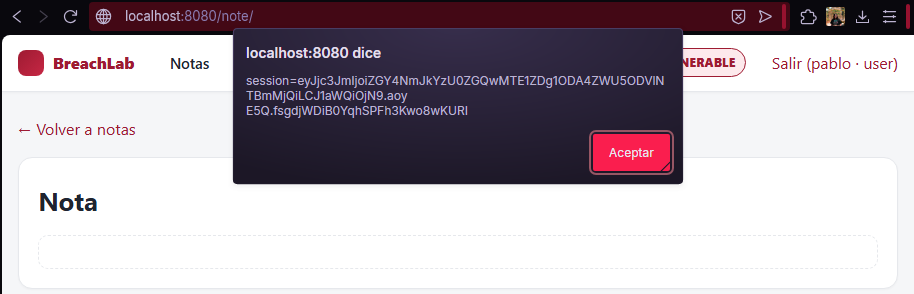
\includegraphics[width=0.75\textwidth]{figures/xss_alert.png}
  \caption{Ejecución del payload XSS al abrir la nota de \texttt{pablo} en
    \breachlab desplegado con Docker: el \texttt{alert()} muestra en claro
    la cookie de sesión, confirmando que el script inyectado se ejecuta en
    el navegador de la víctima.}
  \label{fig:xss-alert}
\end{figure}

\subsection{Evidencia registrada}

A diferencia de otras vulnerabilidades del capítulo, el XSS se ejecuta
enteramente en el cliente y no genera una entrada específica en
\texttt{backend/logs/attacks.log}; la evidencia principal es la ejecución
observable del \texttt{alert} en el navegador. A nivel de API, sí puede
constatarse que el backend acepta y devuelve el payload sin sanear ni
codificar en ningún momento, tal y como quedó guardado al crear la nota:

\needspace{5\baselineskip}
\begin{console}
$ curl -b pablo.txt http://localhost:4321/api/notes/5
{"note":{"content":"<img src=x onerror=\"alert(document.cookie)\">",
         "id":5,"owner_id":3,"title":"Oferta especial"}}
\end{console}

\subsection{Corrección (modo seguro, \texttt{?safe=1})}

En modo seguro, \texttt{note.astro} utiliza \verb|textContent|, por lo que
el payload se muestra como texto literal en lugar de interpretarse como
HTML. Esta corrección se refuerza además con la cabecera
\texttt{Content-Security-Policy} añadida en \texttt{frontend/nginx.conf}
(véase el apartado~\ref{sec:secmisconfig}), que en modo seguro bloquearía igualmente la
ejecución de manejadores de evento inline aunque el contenido se siguiera
insertando por \verb|innerHTML|: dos controles independientes (saneado en el
frontend y cabecera en el servidor) mitigando el mismo fallo, un ejemplo de
defensa en profundidad. Para una discusión más amplia de técnicas de
saneado y codificación de salida, véase la \emph{cheat sheet} de la OWASP
Foundation sobre prevención de XSS~\citelink{OWASPCS-XSS}.

\subsection{Valoración CVSS v3.1}

Vector: \texttt{CVSS:3.1/AV:N/AC:L/PR:L/UI:R/S:C/C:H/I:L/A:N} — Puntuación:
\textbf{7.5 (Alta)}. El atacante necesita una cuenta para crear la nota con
el payload (PR:L) y requiere que la víctima la abra (UI:R). El alcance se
marca como modificado (S:C) porque el impacto trasciende el propio
componente vulnerable: la cookie robada compromete la cuenta de la víctima,
una autoridad de seguridad distinta. La cookie de sesión sin
\texttt{HttpOnly} permite secuestro de cuenta (C:H) y el atacante puede
actuar como la víctima dentro del alcance de la aplicación (I:L).

\section{Cross-Site Request Forgery (CSRF)}
\label{sec:csrf}

\subsection{Descripción y ubicación en el código}

El endpoint \verb|change_password()| (\texttt{backend/api.py}) acepta tanto
GET como POST. En su rama vulnerable no exige token CSRF alguno; en la rama
segura exige método POST y que el parámetro \texttt{csrf} coincida con el
guardado en la sesión del usuario (\verb|session['csrf']|).

\subsection{Explotación}

\begin{enumerate}
\item Se inicia sesión como víctima (por ejemplo, \texttt{marina}) en el
  navegador.
\item Se sustituye \texttt{LAB\_HOST} en \texttt{csrf\_poc.html} por el host
  del laboratorio (por ejemplo, \texttt{localhost:8080}).
\item Se abre \texttt{csrf\_poc.html}: la contraseña de \texttt{marina}
  cambia a \texttt{hackeada123}.
\item Se verifica cerrando sesión y comprobando que la contraseña antigua ya
  no es válida y que la nueva sí lo es.
\end{enumerate}

\begin{figure}[htbp]
  \centering
  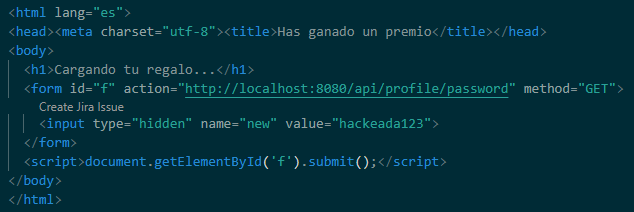
\includegraphics[width=0.7\textwidth]{figures/csrf_poc_html.png}
  \caption{\texttt{csrf\_poc.html} con \texttt{LAB\_HOST} ya sustituido por
    \texttt{localhost:8080}: un formulario GET oculto que se autoenvía en
    cuanto se carga la página.}
  \label{fig:csrf-poc-html}
\end{figure}

\begin{figure}[htbp]
  \centering
  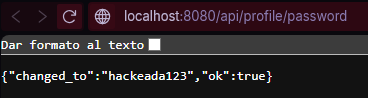
\includegraphics[width=0.55\textwidth]{figures/csrf_poc_abierto.png}
  \caption{Resultado al abrir \texttt{csrf\_poc.html} en el navegador con la
    sesión de \texttt{marina} activa: el formulario se autoenvía y la API
    responde confirmando el cambio (\texttt{ok:\ true}, nueva contraseña
    \texttt{hackeada123}), sin que ella lo haya autorizado.}
  \label{fig:csrf-poc-abierto}
\end{figure}

El detalle clave de esta prueba de concepto es que la cookie de sesión se
configura como \texttt{SameSite=Lax} (\texttt{backend/api.py}). Con esta
política, un subrecurso de otro origen (por ejemplo, un \verb|<img>|) no
envía la cookie, pero una navegación de nivel superior por GET sí la envía;
por ello, \texttt{csrf\_poc.html} utiliza un formulario GET que se
autoenvía, en lugar de un \verb|<img>|. La conclusión relevante para la
memoria es doble: los cambios de estado no deben implementarse nunca
mediante GET, y \texttt{SameSite} por sí solo no es una protección
suficiente frente a CSRF, tal y como demuestra el endpoint seguro, que
exige además un token.

\begin{figure}[htbp]
  \centering
  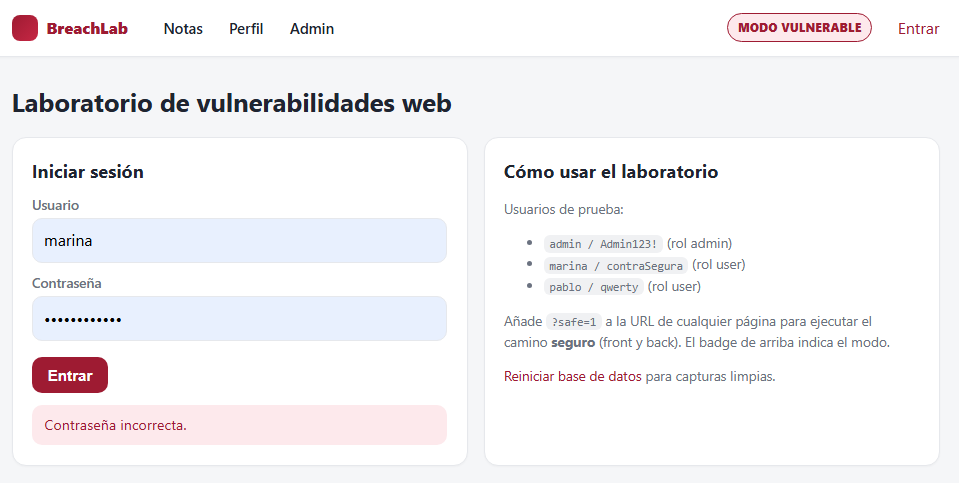
\includegraphics[width=0.6\textwidth]{figures/contrasena-cambiada.png}
  \caption{Verificación del ataque: tras el CSRF, un intento de inicio de
    sesión de \texttt{marina} con su contraseña original
    (\texttt{contraSegura}) es rechazado con «Contraseña incorrecta».}
  \label{fig:contrasena-cambiada}
\end{figure}

\needspace{12\baselineskip}
\subsection{Evidencia registrada}

El cambio de contraseña no autorizado se registra con
\verb|event=csrf_exploited|, incluyendo el usuario, el método utilizado y la
nueva contraseña; el mismo endpoint en modo seguro registra
\verb|event=csrf_blocked| cuando el token no coincide:

\begin{console}
mode=vulnerable ip=127.0.0.1 event=csrf_exploited user=marina
  method=GET new_password=hackeada123
mode=seguro     ip=127.0.0.1 event=csrf_blocked user=marina method=POST
\end{console}

La línea \texttt{event=csrf\_exploited} corresponde a la explotación real en
un navegador (figuras~\ref{fig:csrf-poc-html} y~\ref{fig:csrf-poc-abierto}),
en la que el navegador adjunta la cookie de \texttt{marina} de forma
automática al abrir \texttt{csrf\_poc.html}, sin que ella lo autorice en
ningún momento; la línea \texttt{event=csrf\_blocked} se generó repitiendo
la misma petición sobre el endpoint seguro.

\subsection{Corrección (modo seguro, \texttt{?safe=1})}

En modo seguro, una petición GET al endpoint responde 405 (Método no
permitido) y una petición POST sin el token correcto responde 403 (Token
CSRF inválido). El formulario legítimo de la página de Perfil sí incluye el
token obtenido de \texttt{/api/me}, por lo que el cambio de contraseña
realizado por el propio usuario continúa funcionando con normalidad. El
patrón aplicado corresponde al recomendado por la OWASP Foundation en su
\emph{cheat sheet} de prevención de CSRF~\citelink{OWASPCS-CSRF}: un token
impredecible, ligado a la sesión del usuario y verificado en el servidor
antes de aplicar cualquier cambio de estado.

\subsection{Valoración CVSS v3.1}

Vector: \texttt{CVSS:3.1/AV:N/AC:L/PR:N/UI:R/S:U/C:N/I:H/A:N} — Puntuación:
\textbf{6.5 (Media)}. El atacante no necesita cuenta propia (PR:N), solo que
la víctima tenga sesión activa y abra la página maliciosa (UI:R). El impacto
se concentra en la integridad (I:H), al permitir cambiar la contraseña de la
víctima sin su consentimiento, lo que equivale a una apropiación de cuenta.

\section{Fallos de autenticación}
\label{sec:auth}

\subsection{Descripción y ubicación en el código}

La rama vulnerable de \verb|login()| combina tres debilidades: comparación
de contraseñas en texto plano, ausencia de límite de intentos y mensajes de
error que permiten saber si un usuario existe. La rama segura aplica
hash de contraseñas, bloquea la cuenta tras \verb|MAX_INTENTOS=5| fallos
consecutivos (HTTP 429) y responde siempre con el mismo mensaje genérico.

\subsection{Explotación}

Enumeración de usuarios: la aplicación responde «El usuario no existe» ante
un usuario inexistente y «Contraseña incorrecta» ante un usuario válido con
contraseña errónea, lo que permite confirmar la existencia de una cuenta sin
conocer su contraseña.

Fuerza bruta con lista de contraseñas comunes: \texttt{pablo} utiliza la
contraseña real \texttt{qwerty}, presente en cualquier diccionario básico de
contraseñas débiles:

\begin{console}
for p in 123456 password qwerty admin letmein; do
  echo -n "$p -> "
  curl -s -o /dev/null -w "%{http_code}\n" -X POST http://localhost:8080/api/login \
    -H 'Content-Type: application/json' -d "{\"username\":\"pablo\",\"password\":\"$p\"}"
done   # el 200 (con "qwerty") es la contrasena correcta
\end{console}

Al no existir límite de intentos, el bucle anterior recorre las cinco
contraseñas sin bloqueo alguno, obteniendo un código 200 al probar
\texttt{qwerty}.

\subsection{Evidencia registrada}

Cada intento fallido se registra con \verb|event=login_fail|, incluyendo el
contador de intentos y si el usuario existe o no
(\verb|enumerado=true/false|); el acierto se registra con
\verb|event=login_ok|:

\begin{console}
mode=vulnerable event=login_fail user=noexiste enumerado=False
mode=vulnerable event=login_fail user=pablo    enumerado=True
mode=vulnerable event=login_fail user=pablo enumerado=True query=...password = '123456'
mode=vulnerable event=login_fail user=pablo enumerado=True query=...password = 'password'
mode=vulnerable event=login_ok   user=pablo    query=...password = 'qwerty'
\end{console}

\subsection{Corrección (modo seguro, \texttt{?safe=1})}

Tras 5 intentos fallidos sobre el mismo usuario, la API responde HTTP 429
con el mensaje «Cuenta bloqueada temporalmente», y todo fallo de
credenciales, exista o no el usuario, devuelve el mismo mensaje genérico
«Credenciales inválidas»:

\begin{console}
mode=seguro event=login_fail user=marina intentos=1
mode=seguro event=login_fail user=marina intentos=2
mode=seguro event=login_fail user=marina intentos=3
mode=seguro event=login_fail user=marina intentos=4
mode=seguro event=login_fail user=marina intentos=5
\end{console}

El sexto intento, que responde HTTP 429, no aparece en el bloque anterior:
al reproducir esta secuencia se ha detectado que la respuesta 429 en sí
misma no invoca \verb|log_event()|, quedando constancia de ella únicamente en el
log de acceso HTTP de Werkzeug, no en el registro de eventos de seguridad.
Es una limitación menor no documentada hasta ahora, que se recoge como
línea de trabajo futuro en el capítulo~\ref{cap:conclusiones}.

\subsection{Valoración CVSS v3.1}

Vector: \texttt{CVSS:3.1/AV:N/AC:L/PR:N/UI:N/S:U/C:L/I:N/A:N} — Puntuación:
\textbf{5.3 (Media)}. El vector puntúa la fuga de información que permite
diferenciar un usuario inexistente de una contraseña incorrecta (C:L),
combinada con la ausencia de bloqueo tras varios fallos. Puntúa el fallo en sí mismo; encadenado con una
contraseña débil real, y el resultado
práctico es una toma de cuenta completa, comparable en severidad al vector
de la inyección SQL. Esta cadena de explotación se documenta como agravante
y se retoma en el capítulo~\ref{cap:caso-estudio}.

\section{Control de acceso roto (IDOR)}
\label{sec:idor}

\subsection{Descripción y ubicación en el código}

\verb|note_get()| (\texttt{backend/api.py}) recupera cualquier nota por su
identificador numérico sin comprobar, en su rama vulnerable, si el usuario
autenticado es su propietario. \verb|admin()| presenta el mismo problema a
nivel de rol: no verifica que el usuario tenga rol \texttt{admin} antes de
devolver la lista completa de usuarios, incluidas sus contraseñas.

\subsection{Explotación}

IDOR: iniciando sesión como \texttt{marina} y solicitando la nota con
\texttt{id=3} (propiedad de \texttt{pablo}), se obtiene su contenido
íntegro:

\begin{console}
$ curl -b marina.txt http://localhost:4321/api/notes/3
{"note":{"content":"Contraseña de mi correo: hunter2","id":3,
         "owner_id":3,"title":"No leer!"}}
\end{console}

Escalada de privilegios: accediendo a la sección Admin con la cuenta de
\texttt{marina} (rol \texttt{user}), se visualiza el panel completo,
incluidas las contraseñas de todos los usuarios, sin verificación de rol
alguna:

\begin{console}
$ curl -b marina.txt http://localhost:4321/api/admin
{"users":[{"id":1,"password":"Admin123!","role":"admin","username":"admin"},
          {"id":2,"password":"contraSegura","role":"user","username":"marina"},
          {"id":3,"password":"qwerty","role":"user","username":"pablo"}]}
\end{console}

La misma respuesta, vista desde la interfaz en lugar de la API en crudo,
resulta más clara sobre el impacto real del fallo: cualquier
usuario autenticado, sin ser \texttt{admin}, ve en pantalla la contraseña de
todos los demás.

\begin{figure}[htbp]
  \centering
  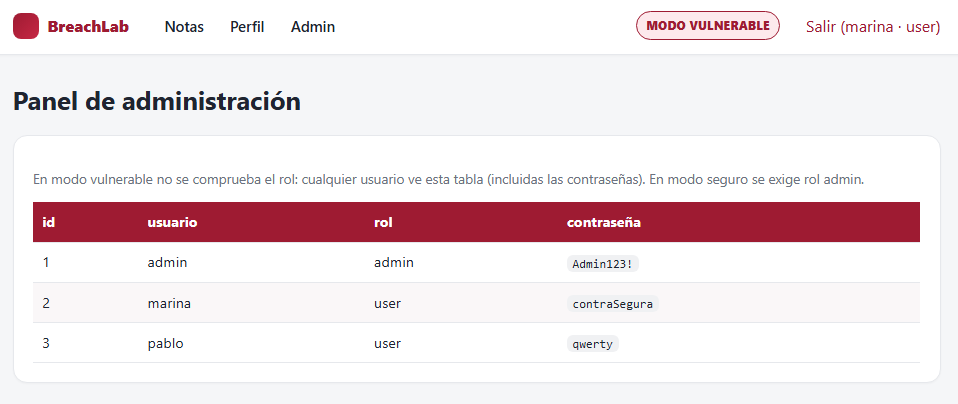
\includegraphics[width=0.75\textwidth]{figures/admin-vulnerable.png}
  \caption{Panel de administración accedido con la cuenta de \texttt{marina}
    (\texttt{user}) modo vulnerable: se muestran las contraseñas en
    claro de los tres usuarios, sin comprobación de rol.}
  \label{fig:admin-vulnerable}
\end{figure}

\subsection{Evidencia registrada}

El acceso a una nota ajena se registra con
{\footnotesize\texttt{event=idor\_exploited user=marina note\_id=3 owner\_id=3}};
el acceso al panel de administración sin ser admin se registra con
\verb|event=admin_privesc|:

\needspace{5\baselineskip}
\begin{console}
mode=vulnerable event=idor_exploited user=marina note_id=3 owner_id=3
mode=vulnerable event=admin_privesc  user=marina role=user
mode=seguro     event=idor_blocked   user=marina note_id=3 owner_id=3
mode=seguro     event=admin_blocked  user=marina role=user
\end{console}

\subsection{Corrección (modo seguro, \texttt{?safe=1})}

En modo seguro, \texttt{/api/notes/3?safe=1} responde 403 si el solicitante
no es el propietario de la nota ni tiene rol \texttt{admin}
(\verb|event=idor_blocked|); el panel de administración responde también
403 si el rol del usuario no es \texttt{admin} (\verb|event=admin_blocked|).

\begin{figure}[htbp]
  \centering
  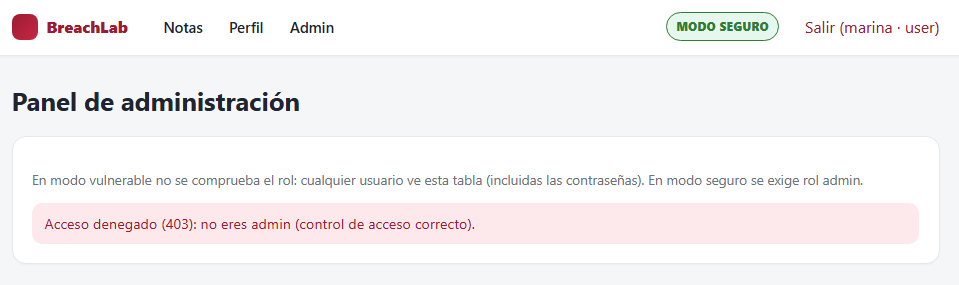
\includegraphics[width=0.75\textwidth]{figures/admin-seguro.png}
  \caption{Panel de administración, con \texttt{marina} y
    \texttt{?safe=1}: acceso denegado (403).}
  \label{fig:admin-seguro}
\end{figure}

\subsection{Valoración CVSS v3.1}

Vector: \texttt{CVSS:3.1/AV:N/AC:L/PR:L/UI:N/S:U/C:H/I:N/A:N} — Puntuación:
\textbf{6.5 (Media)}. Requiere una cuenta de usuario normal (por ejemplo,
\texttt{marina}) para explotarse (PR:L) y expone datos de otros usuarios,
incluidos datos ficticios sensibles como una tarjeta de crédito o una
contraseña de correo (C:H). En el caso del panel de administración, las
contraseñas expuestas habilitan además una escalada de privilegios por
reutilización de credenciales, agravante que se comenta explícitamente
frente al vector base.

\section{Configuración de seguridad insegura (cabeceras HTTP)}
\label{sec:secmisconfig}

\subsection{Descripción y ubicación en el código}

En el bloque \verb|location /| de \texttt{frontend/nginx.conf}, el modo
vulnerable no añade ninguna cabecera de hardening. En modo seguro se añaden
condicionalmente (cuando \verb|$arg_safe = "1"|) las cabeceras
\texttt{Content-Security-Policy}, \texttt{X-Content-Type-Options},
\texttt{X-Frame-Options} y \texttt{Referrer-Policy}.

\needspace{9\baselineskip}
\subsection{Comprobación}

A diferencia del resto de vulnerabilidades de este capítulo, esta
comprobación depende de nginx (\texttt{frontend/nginx.conf}) y solo puede
reproducirse desplegando \breachlab con \texttt{docker compose up --build}:
en modo desarrollo (\texttt{npm run dev}), al no pasar las peticiones por
nginx, ninguna cabecera se añade en ningún modo y la comparación no sería
representativa. Desplegado con Docker, basta con comparar las cabeceras de
respuesta:

\begin{console}
$ curl -sD - -o /dev/null http://localhost:8080/dashboard/
HTTP/1.1 200 OK
Server: nginx/1.31.4
Content-Type: text/html
...

$ curl -sD - -o /dev/null "http://localhost:8080/dashboard/?safe=1"
HTTP/1.1 200 OK
Server: nginx/1.31.4
Content-Type: text/html
Content-Security-Policy: default-src 'self'; script-src 'self';
  style-src 'self' 'unsafe-inline'; object-src 'none'; base-uri 'self'
X-Content-Type-Options: nosniff
X-Frame-Options: DENY
Referrer-Policy: no-referrer
...
\end{console}

\subsection{Relación con el XSS del apartado~\ref{sec:xss}}

Esta vulnerabilidad no se puntúa de forma aislada: la ausencia de estas
cabeceras no es explotable por sí sola, pero amplifica el impacto real de
otras vulnerabilidades. En particular, la CSP del modo seguro
(\verb|script-src 'self'|) bloquearía también los manejadores de evento
inline del payload del apartado~\ref{sec:xss} aunque el contenido se siguiera
insertando por \verb|innerHTML|, mientras que la ausencia de
\texttt{X-Frame-Options} habilita ataques de clickjacking embebiendo el
sitio en un iframe de un dominio de terceros. Se documenta, por tanto, como
un control compensatorio ausente más que como una vulnerabilidad
independiente.

\subsection{Valoración CVSS v3.1}

Como ilustración del riesgo de clickjacking que introduce por sí sola la
ausencia de \texttt{X-Frame-Options}:
\texttt{CVSS:3.1/AV:N/AC:L/PR:N/UI:R/S:U/C:N/I:L/A:N} — Puntuación:
\textbf{4.3 (Media)}.

Resumen de severidad de las vulnerabilidades analizadas:

\begin{table}[htbp]
  \centering
  \small
  \begin{tabular}{lp{5.2cm}cl}
    \toprule
    \tabhead{Vulnerabilidad} & \tabhead{Vector CVSS v3.1} & \tabhead{Puntuación} & \tabhead{Severidad} \\
    \midrule
    Inyección SQL (\S\ref{sec:sqli})             & \path{AV:N/AC:L/PR:N/UI:N/S:U/C:H/I:H/A:N} & 9.1 & Crítica \\
    XSS DOM (\S\ref{sec:xss})                    & \path{AV:N/AC:L/PR:L/UI:R/S:C/C:H/I:L/A:N} & 7.5 & Alta    \\
    CSRF (\S\ref{sec:csrf})                      & \path{AV:N/AC:L/PR:N/UI:R/S:U/C:N/I:H/A:N} & 6.5 & Media   \\
    Fallos de autenticación (\S\ref{sec:auth})   & \path{AV:N/AC:L/PR:N/UI:N/S:U/C:L/I:N/A:N} & 5.3 & Media   \\
    IDOR (\S\ref{sec:idor})                      & \path{AV:N/AC:L/PR:L/UI:N/S:U/C:H/I:N/A:N} & 6.5 & Media   \\
    Configuración insegura* (\S\ref{sec:secmisconfig}) & \path{AV:N/AC:L/PR:N/UI:R/S:U/C:N/I:L/A:N} & 4.3 & Media   \\
    \bottomrule
  \end{tabular}
  \caption{Vectores y puntuaciones CVSS v3.1 de las vulnerabilidades de
    \breachlab (*el vector del apartado~\ref{sec:secmisconfig} ilustra el
    riesgo de clickjacking derivado; se documenta como control
    compensatorio ausente, no como vulnerabilidad independiente).}
  \label{tab:cvss-resumen}
\end{table}
